\section{Literature Review}
\label{sec:lit-review}
% introduction goes here
% define topic 
The topics reviewed in this section touch on various fields relating to the development of the VRDAVis system.
This involves reviewing other systems which attempt to create real-time and interactive visualisations of large volumetric datasets. 
As well as other topics which support this process such as analytics, visualisation and rendering strategies.
% These topics relate to the field of virtual reality (VR), visual analysis, data visualisation, and volumetric graphics rendering strategies.
% reasons 
With the goal to gather insight into techniques and methodologies that can enrich the VRDAVis system. 
% but does not go into depth over how the data files are pre-processed instaed it discusses why the pre-processed file are useful 
% Finally, a survey of current systems employed in the visualisation of big data in astronomy is conducted. 
% It's important to note that the scope is confined to these specific themes, predominantly focusing on methodologies and best practices pertinent to the implementation of VRDAVis.
\subsection{Virtual Reality}
\label{sec:virtual-reality}
% what is virtual reality?
VR immerses users in an interactive digital environment using a head-mounted display.
The ``ultimate display" as described by Ivan Sutherland is a theoretical human-computer interaction device that simulates a reality that is realistic to the point where a person cannot tell the difference between actual reality and the simulated reality~\cite{Sutherland1965}.
This level of immersion in a completely new world was an appealing idea even before the technological inception of a device that was even remotely capable of achieving it.
The virtual world appears realistic to a human through the use of stereoscopic displays and sound.
Stereoscopic displays present each eye with a different image for the user to experience simulated depth.
Also, gives the user the ability to interact with the virtual objects in a realistic way with tactile feedback.
% This includes not just observing the virtual world, 
% The concept VR follows the ideals of the ``ultimate display" has shaped the ideas and ideals for VR technology, where with every iteration of the technology it becomes evermore achievable. 
Since the 1960s, the concept of virtual VR headsets has evolved significantly. 
One of the earliest examples dates back to this era, with Morton Heilig's Telesphere Mask~\cite{Heilig1994} which introduced the notion of a head-mounted display. 
It offered wide vision, a stereoscopic 3D display, and stereo sound; it was later augmented by the introduction of a motion tracking feature in 1961.
Over time, various entities, including NASA, Sega, Nintendo, Apple, and Google, have experimented with VR technology. 
Recent advancements have been marked by Oculus, now owned by Meta, which is releasing affordable VR headsets aimed at mass market consumption, particularly targeting the entertainment sector.
However, VR technology is in the process of being adopted in other industries such as education, retail, transportation, energy, consulting, insurance, healthcare, and sports.

\begin{figure}
    \centering
    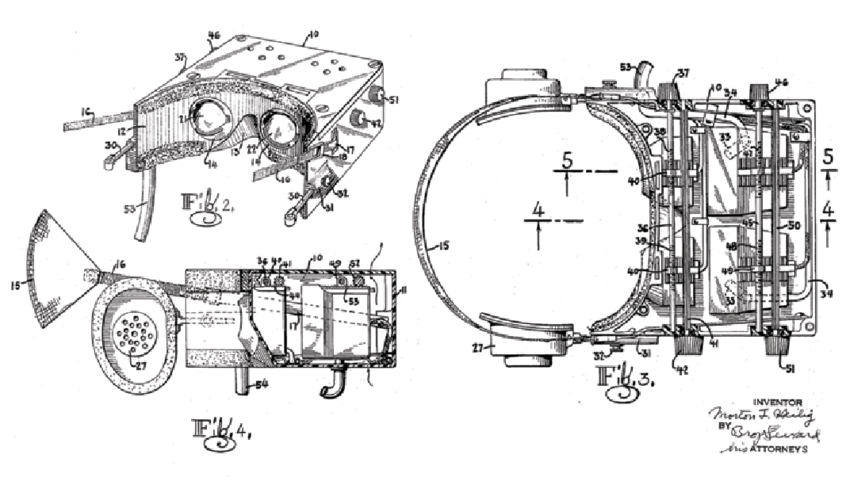
\includegraphics[width=\linewidth]{figures/telesphere-mask.png}
    \caption{Morton Heilig's patent for the Telesphere Mask~\cite{Heilig1994}, note the resemblance to contemporary headset design, such as the Meta Oculus Quest and the Apple Vision Pro.}
    \label{fig:telesphere}
\end{figure}

% what does it do?
%\cite{Wohlgenannt2020} % add othe citations mentioned in this paper
VR uses immersive technology to simulate interactive virtual environments where users feel physically present~\cite{Wohlgenannt2020, Bowman2007}.
This is done through the construction of a real or imagined environment, which blocks the real world from the user.
It also incorporates interaction methods such as controllers and motion tracking for the user to interact with the environment~\cite{Brooks1999, Barfield2000}.

% other VR tecnologies
% augmented reality (AR), augmented virtuality (AV), terms also refered to as mixed reality (MR) superimposes virtual agents over the real world in real-time (added digital information to physical reality)
% the term extended reality (XR) is a term used to refer to all the possible combinations of  real-and-virtual environments and human–machine interactions generated by computer technology and wearables
%  used as a umbrella term for their combined use

\begin{figure}
    \centering
    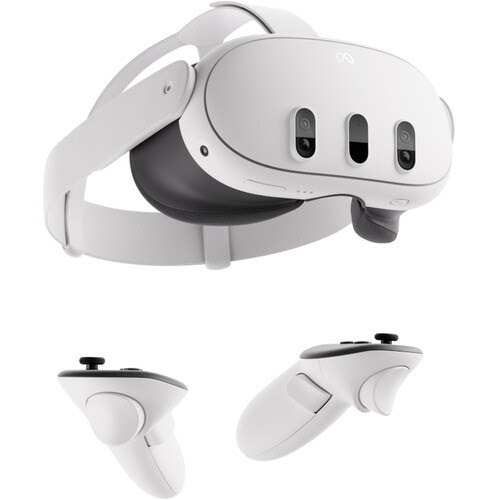
\includegraphics[width=0.6\linewidth]{figures/oculus-quest.jpg}
    \caption{An example of one of the latest iterations of VR technology, Meta's Oculus Quest 2. It can be considered as a extended reality (XR) headset as it can host VR environments while also incorporation augmented reality (AR) features.}
    \label{fig:oculus-quest-2}
\end{figure}

VR experience can be evaluated according to three key properties: presence, interactivity, and immersion~\cite{Walsh2002}.
% presense refers to the sense of physically being somewhere other where someone actually is
Presence refers to the sense of being physically somewhere.
Within a virtual environment, the presence of the user is simulated by capturing their senses, using visual, audio, and tactile simulations~\cite{Sanchez2005}.
% visual, ausio and tactil(haptics) realism is an important factor for presense in a virtual environment
% as well as virtual body representation and body engagement
The feeling of being present in virtual environments arises from the way that a user perceives and processes information from their surroundings, both in their conscious and subconscious environment~\cite{Barfield2000}.
% Some factors which contribute to how present a user feels in a virtual environment are: the virtual environment, communication medium, the individual user, any disturbances from the real world and, the task or tasks which the user performs.
% there are factors which contribute to presense
%   the computer and virtual environment
%   the communication medium
%   the individual
%   disturbances from the real-world environment
%   the task
The sense of presence that a user feels is difficult to quantify, as it can be measured in objective and subjective ways.
Subjective measurement comes from the level of realism in the virtual environment.
As VR technology improves, the level of realism VR headsets are able to display improves with it.
% Subjective measures of presense
%   realism is an essential part of presense in a virtual environment
%   as the technology used in contemporary VR headsets improve so does the realism and sense of presense within the environment
The objective measure of presence observes physical indicators in the user; these indicators include heart rate, dilation of the pupils, blink responses, and muscle tension.
% Objective measures of presense
%  physical indicators in a test subject (Heart rate, pupil dilation, blink responses, and possibly muscle tension)
Some more objective measurements include the extent to which physically reality is excluded from the virtual one, the number of the user's senses that are captured by the virtual reality, the extent of the field of view, the resolution and quality of the displays used, and how the user's body movements match up against their movements in the virtual world~\cite{Sanchez2005, Barfield2000}.
% objectively measurable 
%   inclusiveness - the extent to which reality is exculded
%   extensiveness - the range of sensory modalities
%   surrounding - the size of the feild of view
%   vivedness - the richness, resolution, and quality of the displays
%   matching - the extet to which proprioceptive feedback on body movementsin aligned with display information
% Immersion can be quantifiable judged through the assessment of the inclusively, extensiveness, display size and resolution of display technology~\cite{Barfield2000}.
% The aspect of inclusively refers to how much of the real world is the display able to block out from the vision, extensiveness refers to how many senses the technology encapsulates, such as taste, touch, sight, smell, and hearing.
% The display size judges how panoramic the display is and the resolution refers to the level of resolution or number of pixels on the display.
%   inclusive - the degree to which the stimuli from the real world are excluded from the user
%   extensive - the number of sensory modalities accommodated by the system
%   surroundings - how panoramic the displays are
%   vivid - the resolution of the displays
Interactions in the real world are naturally as good as they could possibly be according to both subjective and objective measurements of presence.
Human senses have specifically adapted for perceiving and interacting in the real world, and therefore it is difficult to simulate the same level of realism digitally.

VR Interactivity refers to how effectively a user can manipulate the virtual environment in real time~\cite{Steuer2000}.
In interactive systems, users have agency and control over various elements within the virtual environment, which allows them to make decisions, perform actions, and influence outcomes with their interactions.
This can range from simple actions like clicking buttons or navigating menus to more complex interactions such as manipulating objects, and altering parameters. 
The level of interactivity correlates with the user's sense of immersion and engagement, as it enables them to influence the environment and participate actively in the experience according to their preferences, goals, and intentions.
% interactivity refers to the extent to which a user can manipulate their environment in real time
Interactivity is a key factor as it affects the level of presence the user feels within the environment and directly influences the user's sense of presence. 
% interactivity can affect the presence the user feels within the environment (body engagement)
 
Immersion in VR is more complicated than presence and interactivity.
% It can be classified as subjective involvement which involves cognitive, emotional, sensory-motor, and spatial immersion.
Immersion can be described as subjective involvement, encompassing various dimensions of a user's experience~\cite{Nilsson2016}. 
However, there are many facets of immersion.
Cognitive immersion manifests when a user engages with the content, experiencing satisfaction and fulfilment upon solving complex problems. 
Emotional immersion occurs when a user become emotionally invested in narrative structures, experiencing highs and lows which come with a story. 
Kinesthetic immersion emerges when users receive immediate feedback on their physical actions, which enhances their sense of presence and agency within the virtual environment. 
% The term distal-attribute describes this phenomenon aptly, it is where an individual creates a mental representation of themselves to include the external and virtual worlds.
% For example, when a tool becomes and extension of an individual's body but it is not physically part of it.
% the phenomenon of individuals creating a mental representation of them selves to include in the external and virtual world.
% eg a tool becomes an extension of your body even though it is physically not
Spatial immersion is experienced as users navigate and perform intricate movements, feeling a sense of spatial presence and immersion within the simulated world. 
These dimensions collectively contribute to a rich and immersive user experience across various interactive platforms and media.
%  immersion can also be classifed as subjective involvement
%   cognitive immersion - users feel when they solve complex problems
%   emotional immersion - users feel when narrative structures unfold
%   sensory-motoric immersion - users feel when they receive feedback on movements
%   spatial immersion - users feel when they perform extensive maneuvers/
The sense of presence relates to the perception of the physical environment and is tightly coupled to how immersed the user feels.
Vice versa, the more immersed the user feels in the virtual environment, the easier it is for them to feel present.

While VR systems offer immersive experiences, they face some downsides, notably simulator sickness. 
This condition is caused by to frame rate drops.
Frame rate is the number of images a display such as a screen can cycle through per second.
The rapid succession of frames on the display is what causes the image on the screen to appear to have motion.
When the frame rate is high, the motion on the display appears smooth; low frame rate makes the motion of the image to appear choppy and unpleasant.
It is this choppy movement on the display which leads to a disconnect between user input and display output, which results in feelings of confusion, dizziness, and nausea for some users. 
% Simulator sickness can easily arise from a poorly designed or poorly performing system.
The level of susceptibility to simulator sickness varies between individuals, but has some dependence on a users experience with VR headsets as well as their natural tolerance to being in a VR environment.
Additionally, as the system's performance declines, the immersive element of the experience diminishes, which highlights the sensitivity of VR experiences to hardware performance. 
Users experience disconnect from the environment when any aspect of presence, interactivity, or immersion is compromised.
% A consequence of this disconnect is that a user may experience simulator sickness.
% Thus, the overall experience of a VR system heavily relies on consistent and high-performance hardware to maintain immersion and prevent adverse effects on users.
% the downsides
% simmulator sickness
% frame rate drop produces a disconnect between the user input and the display output causing a feeling of confusion, dizziness and nausea in some users
% the immsersiv element of the experience breaks down as the performance of the system drops
% the experience of a VR system is dependent on the hardware's performance and is incredible sensitive to drops in performance
\subsection{Visual Analytics}
\label{sec:visual-analytics}

Visual analytics is the practice of analysing datasets using visual representations of the data, these representations are the individual data points of the dataset mapped using a particular visualisation strategy \cite{Bikakis2018}. 
% Offer benefits such as visual perception, interactive exploration, improved understanding, informed steering, and intuitive interpretation~\cite{Li2016}.

Visualisations facilitate the emergence of patterns as they are explored by analysts, typically domain experts, enhancing accessibility, interpretation, and meaningful analysis of data~\cite{Lowe2020, Tukey1977} through interactive engagement with diverse tools.
These visualisations are made with goals in mind, which can be exploitative, confirmatory or for presentation~\cite{keim1997}.
Exploitative analysis involves undirected interaction with data which does not have a hypothesis attached to the exploration.
This type of analysis is done to construct a possible hypothesis relating to the data.
In contrast to confirmatory analysis has a more goal-oriented approach; the purpose of the exploration or examination of the data is to confirm or reject a hypothesis.
This is for the purpose of either confirming or rejecting the hypothesis.
The goal of presentation differs from the goal of a hypothesis where it is only concerned with the technique it uses to present the data to best represent the facts it wishes to communicate.
Human analysts are naturally equipped with sophisticated pattern recognition abilities~\cite{Hassan2011, Taylor2015, Sneiderman1996}, and applying these skills while interacting with data visualisations facilitates knowledge extraction~\cite{Caldarola2017, Yi2007, Becker1987, Glueck2014, Bikakis2018, Muhlbacher2014, Shneiderman2008}.
Large datasets within the Big Data field require analysts' cognitive abilities to make sense of the data, using perceptual grouping, image segmentation, and object recognition~\cite{Lowe2020}.
These skills allow elements such as clustering, outliers, patterns, and correlations between characteristics become apparent.
A visualisation can communicate the essence of a dataset quickly and effectively regardless of size~\cite{Fisher2012}.
The aim of visual analytics is to support the analysts' analytical reasoning and research with interactive visualisations of datasets~\cite{Tufte1983, Ali2016, Becker1987}.

For the users to explore the visualised datasets there must be some interactions they can perform to affect the representation~\cite{Yi2007} without interaction the representation would be a static image~\cite{Becker1987}.
Static images do offer value in visual analytics, but this value is limited once the dataset exceeds a certain size and the granularity of the data becomes too fine.
Interactions performed on the representation must produce an instantaneous change in the visualisation to maintain the user's attention.
There is a threshold of 10ms or less between interaction input and response to facilitate an uninterrupted dialog between the user and the data~\cite{Glueck2014, Li2016, MacKenzie1993, Muhlbacher2014}.
% \cite{Li2016, Zhao2017, MacKenzie1993, Becker1987}
% Visualisation system should retreive data fast enough so that the analist does not lose interest or lose a train of thought (focus and momentum)
% minimise the user's waiting time as much as possible

\subsubsection{Progressive visualisation}
As a user analyses a representation of the dataset, the visualisation should allow the user to steer the appearance of the visualisation through interaction and should also allow them to drill down into areas of interest within the data.
This is the process of progressive visualisation where initially a low fidelity representation is displayed and as it is explored, higher fidelity data is brought into the visualisation~\cite{Zhao2017, Ahrens2005, Rosenbaum2009, Li2016, Tufte1983}.
% To understand the context of the data it is more important to get a broad overview of the data than exact figures.
The user steers the visualisation's progression through the data and the visualisation changes as they explore the data~\cite{Zhao2017, Muhlbacher2014, Fisher2012}.
% Displaying  a  low  fidelity  representation  prior  to  loading  a high  fidelity  version  has  long  been  utilised  to  ensure  responsive  interaction  [4,14,19]. % check refs
% \cite{Zhao2017}
% progressive visualisation / progressive visual analytics
% produce intermediate results of the visualisation as the user explores the dataset
% the dataset can be sampled randomly to make these progressive visualisation or it can be arranged in a heirchical format.
The data stored at different levels of fidelity are pre-processed into a hierarchical order so that required data can be found easily~\cite{Glueck2014}.
% This method of storing data aligns with the exploration process the user undergoes when interacting with the visualisation~\cite{Rosenbaum2009}, the whole dataset is first shown to the user, and as they explore the model increases in resolution as they zoom in on areas of interest.
Pre-processing data used for visualisation can dramatically improve the user experience~\cite{Shneiderman2008}.
% Visualisation tools should give the user a high level overview initially and subsequently load more data as the user explores areas of interest~\cite{Li2016, Tufte1983}.
Some of the visualisation tools for interactions should include scaling, translation, rotation, filter, overview, and detail-on-demand~\cite{Zhao2017, Becker1987, Sneiderman1996, keim1997, Baracaglia2019, Ferrand2016}. 
%overview first, zoom and filter, then details on demand
% In three-dimensional datasets these interaction translation, rotation, croping, measurement and transparency \cite{Baracaglia2019, Ferrand2016}.

Scaling data correctly is important for lower-powered devices such as the VR headset and personal laptop computers, as they have comparatively fewer computational resources available.
The visualisation of points which translates to a size which is smaller than a single pixel on a screen is a waste of resources and should be minimised~\cite{Li2016, ertl1999}.

% \cite{Fisher2012}% information visualization, large amounts of quantitative data can be shown in a limited space
% graphical display extended to visualisations should
%   show the data
%   induce the viewer to think about the substance rather than about methodology, graphic design, the technology of graphic production, or something else
%   avoid distorting the message in the data
%   present a large amount of data in a small space
%   make large sets coherent
%   encourage the eye to compare different pieces of data
%   reveal the data at several levels of detail, from broad overview to fine structure
%   serve a reasonably clear purpose: description, exploration, tabulation, or decoration
%   be closely integrated with the statistical and verbal descriptions of the dataset

\subsubsection{Virtual reality in visual analytics}
Human eyes are naturally suited for three-dimensional space are more in accustomed to interacting with three-dimensional objects and VR simulates this interaction~\cite{Ferrand2018, Abidi2017}.
VR headsets provide an inexpensive and portable environment for multi-dimensional visualisations, which provides the ability to interact with the visualisation.
Three-dimensional data visualised in three-dimensional space grant a holistic view of the of the data~\cite{Ferrand2016, Farr2009}.
An effective visualisation bridges the gap between the data contained in datasets and the human ability to extract knowledge.
The stereoscopic environment produced by a VR headset such as the Oculus Quest 2 allows the user to see the data with a perception closer to a real-world environment, fostering user friendly interaction which resembles interaction in the real world.
% The VR headset also track the user's movement adding an extension of self into the VR environment for increased immersion
% While building the experimental system E0102-VR~\cite{Baracaglia2019} some insights were found involving the use of VR for viewing and interacting with multi-dimensional datasets.
% The depth perception provided by VR aids in understanding complex three-dimensional structures and provides means to quickly measure distances and angles in three dimensions.

% \cite{Ferrand2016}
% major challenges faced by astronomers is to digest the large amount of diverse data generated by modern instruments or simulations
% develop visualization tools that allow exploration of all their complexity and dimensions
% interested in displaying the 3D data in actual 3D space, to get a holistic view, in the expectation that this will generate a more correct perception, and help build an intuition, of the data.
% user friendliness - developing interfaces allowing for Natural User Interaction (NUI) in 3D is still an active field of research
% flat display of a desktop or mobile computer, the visualization is limited to 2D views: slices and projections, that have to be flipped through, or a fake 3D view, emulated with tricks like per- spective and shading.
% Stereoscopic 3D can be achieved using dual projectors, that present a slightly different image to each eye
% The 3D displays we are considering here bring something more: the tracking of the viewer (commonly using infrared cameras), which makes the experience distinctively different. First this enables motion parallax, which gives a much stronger depth cue, and second this allows direct interaction with what is being displayed. Depending on the hardware used, one can get the feeling of being fully immersed inside the data cube, as if it was a physical object that we can explore and manipulate.
% 3D displays for Virtual Reality come broadly into two categories: “fish tanks”, systems where the user is looking at a fixed screen or set of screens that define the boundaries of a virtual volumetric screen, and head-mounted displays (HMD), systems where the user is wearing a pair of screens attached directly in front of their eyes.
% serious applications in the medical and architectural fields, with also several experiments in the natural sciences: biology, geology, meteorology.
% ray casting: for each pixel to be rendered on the screen, a ray is cast along the current line of sight, and along this ray the data is retrieved at regularly spaced intervals. The values are accumulated along the line of sight using the standard radiative transfer approximation: the value at a point (understood here as a voxel) is interpreted as both an emissivity (added to the R, G, B channels) and an opacity (using the alpha channel to handle transparency)

% \cite{Ferrand2018}
% visualisation is important for exploring as well as the communication of data
% astronomy uses 3D data sets
% humans are more in tune to interact with 3D objects
% VR facilitates this interacting

% \cite{ertl1999}  hierarchical methods for visualisation of volume data
% basically introduces a hierarchical structure to the volume data so that it takes less time and memory to create a visualisation
% The standard model of this process comprises a pipeline of three stages. The filter stage is a preprocessing step converting the raw input data into visualization data which is usually reduced by operations like sampling, slicing, cropping, etc. The mapper stage performs a mapping of the abstract data fields into a visual representation consisting of geometric primitives like points, lines, surfaces or voxels and associated graphical attributes like color, transparency, texture, etc. The renderer, finally, uses this scene description to generate images by means of 3D graphics APIs such as OpenGL or OpenInventor, possibly exploiting 3D graphics hardware to achieve interactive frame rates.
% the user has to be given control over the threshold letting him choose between a fast visualization of a very crude approximation of the data and an almost perfect representation of the data which took perhaps minutes to compute. This requirement can only be met if not only one compressed version of the data, but a complete hierarchy of representations of the data set at different levels of resolution is available or can be generated on the fly.
% Direct volume rendering tries to convey a visual impression of the complete 3D data set by assigning different color and opacity values to different objects or value ranges within the volume. The resulting image is then computed by taking into account the so-defined emission and absorption effects as seen by an outside viewer. 
% Hierarchical approaches
%   

% \cite{keim1997}
% goals of visualisation
%   explorative analysis
%       start -> data without hypotheses about data
%       process -> interactive, undirected search for structures, trends, etc.
%       result -> visualisation of data, which provides hypotheses about data
%   confirmative analysis
%       start -> hypotheses about data
%       process -> goal orienatated examination of the hypotheses
%       result -> visualisation of data,which allows the confirmation or rejection of the hypotheses
%   presentation
%       start -> facts to be presented
%       process -> choice of presentation technique
%       result -> high quality visualisation of data presenting facts

% classifications of data visualisation techniques
%   geometric techniques -> scatterplots, landscapes, parallel coordinates
%       visualization of geometric transformations and projections of the data.
%   icon-based techniques -> stick figures, color icons, shape-coding
%       Visualization of the data values as features of icons.
%   pixel-orientated techniques -> spiral- , axes-techniques, recursive pattern techniques
%       each attribute value is represented by one colored pixel ( the value ranges of the attributes are mapped to a fixed colormap)
%       the attribute values for each attribute are presented in separate subwindows
%   hierarchical techniques -> treemap, dimensional stacking
%       Visualization of the data using a hierarchical partitioning into subspaces.
%   graph-based techniques -> basic graphs
%       Visualization of large graphs using techniques to convey the meaning of the graph clearly and quickly.

% Dynamic interaction techniques
% Dynamic generation of the visualizations or interaction with the visualization for a more effective exploration of the data
%   data-to-visualisation mapping
%   projections
%   filtering (selection, querying)
%   linking, brushing
%   zooming
%   detail on demand

% data pre-processing techniques
%   Dimension reduction techniques
%       principal component analysis -> Determines a minimal set of principal components (linear combinations of the original dimensions) which explain the main variations of the data.
%       factor analysis -> Determines a set of unobservable common factors which explain the main variations of the data. The original dimensions are linear combinations of the common factors.
%       Multidimensional Scaling -> Uses the similarity (or dissimilarity) matrix of the data as defining coordinate axes in multidimensional space. The Euclidean distance in that space is a measure of the similarity of the data items
%       fatsmap -> Fastmap also operates on a given similarity matrix and iteratively reduces the number of dimensions while preserving the distances as much as possible.
%   Subsetting techniques
%       (Set of Data Items -> Subset of Data Items)
%       Sampling (determines a representative subset of the database
%       Querying (determines a certain, usually a-priori fixed subset of the database)
%   Segmentation techniques
%       (Set of Data Items -> Set of (Set of Data Items)
%       Segmentation based upon attribute values or attribute ranges
%   Aggregation Techniques
%       (Set of Data Items -> Set of Aggregate Values
%       Aggregation (sum, count, min, max, ...) based upon attribute values, opological properties, etc.
%       Visualizations of Aggregations: Histograms, Pie Charts, Bar Charts, Line Graphs, etc
\subsection{Data Visualisation}
\label{sec:data-visualisation}
This section will summaries the different techniques and strategies used to create visualisations of astronomy data cubes or any volumetric data. 
% explain volumetric data
Volumetric datasets can be thought of as data cubes as they have data along the \textit{x}-,\textit{y}- and \textit{z}-axes. 
They are commonplace in fields such as astronomy, medicine, oceanography, molecular modelling, and engineering.
Data cubes can be described as a set of samples \textit{(x, y, z, v)}, where the value of \textit{v} is some property of data at the three-dimensional coordinates \textit{(x, y, z)} \cite{Kaufman2000}.
A point within a data cube is a three-dimensional pixel and is referred to as a voxel or volume pixel~\cite{Kaufman1996}.
In astronomy datasets \textit{x} and \textit{y} are used for spatial information where the third axis, \textit{z}, is usually a red-shift value, not distance.
The steps through the \textit{z}-axis are refereed to as channels and the number of channels on the \textit{z}-axis depends on the velocity resolution and bandwidth of the receiver~\cite{Taylor2015}.
% the high dynamic range makes assigning colours difficult
% a representation of a point in a three-dimensional dataset is called a voxel or volume pixel which is essentially a three-dimensional pixel and has an x, y, and z coordinate
% These datasets are essentially represented as a three-dimensional scatter plot.
The data is a representation of a measurable property of astrophysical phenomenon, and can be represented as binary values or values within a range.
% the data can be binary, represented as zeros and ones or be multivalued and be a representation of some measurable property
% start by stating why visualisation is important
% what does visualisation do for astronomy data

% -------------
Data visualisation is the presentation of data as a static or interactive image~\cite{Bikakis2018}.
Visualisation is imperative to making sense of abstract datasets such as those prevalent in radio astronomy research ~\cite{Glueck2014, Yang2017},
and is important for the exploration of data and the communication of findings~\cite{Ferrand2018}.
Visualisations allow enormous amounts of quantitative data to be shown in a limited space, while also maintaining the message contained within the dataset~\cite{Fisher2012}.
% Allows the user to see the data without concerning themselves with the methodology or the technology of the graphical production.
% How astronomers use their skills in visual analytic to extract knowledge from these visualisation is inspected further in Section~\ref{visual-analytics}.
Data visualisation has some distinct objectives~\cite{Norris1994, McReynolds2005, Hassan2011}: 
\begin{itemize}
    \item Allow the user to explore the data and obtain a deeper understanding~\cite{Bikakis2018}.
    \item Expose features within the dataset which would otherwise have remained hidden.
    \item Obtain quantitative results from the data, and communicate the results to others.
\end{itemize}

\begin{figure*}
    \centering
    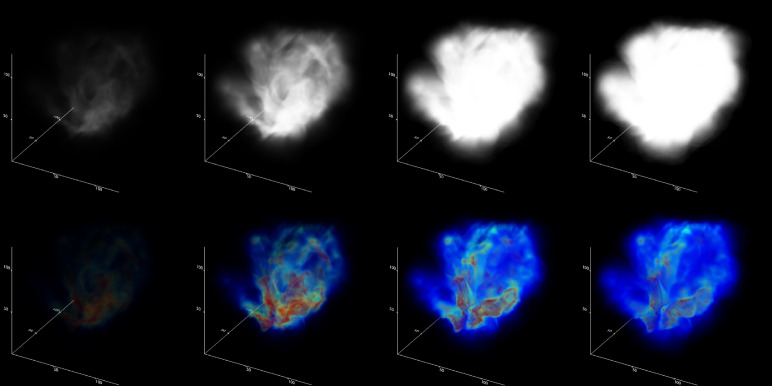
\includegraphics[width=1\linewidth]{figures/volume.jpg}
    \caption{An astronomy dataset visualisation generated by Frelled~\cite{Taylor2015} depicting how the addition of colour and opacity applied to the voxels effectively exposes hidden structures within the dataset. It shows how various ranges of opacity affect the visualisation but also how colour adds to its readability.}
    \label{fig:volume}
\end{figure*}

% Visualisation plays an integral role in allowing the visualisation to be interactively steered,
% the importance of visualisation and interaction for visual analysis is discussed further in Section \ref{visual-analytics}.

% visualisation challenges
There are certain characteristics present in the data which make visualisation difficult~\cite{Hassan2011}.
The datasets produced by astronomy data gathering instruments produce massive amounts of data, giga-bytes to peta-bytes, large enough to fill the memory of multiple conventional desktop computers.
This makes the datasets difficult to manage and process for visualisation.
There is no dominant file type used to represent astronomy data, which makes the development of a generic visualisation tool difficult.
Conventionally FITS files~\cite{wells1979} have been used to represent data cubes.
The cubes are divided up into slices along the \textit{z}-axis. 
Each of the these slices can be visualised as an image consisting of pixels with an \textit{x} and \textit{y} coordinate.
A user can move through slices of a data cube sequentially and can be played through like frames in a movie.
A major downside of visualising the data in this manner is that it does not let the user get an impression of how the dataset looks as a whole.
Therefore, limiting how quickly and effectively a user can construct a mental model and begin extracting insight~\cite{Norris1994}.
% bottleneck between human and machine where it is difficult for the user to construct model of the information in their mind in a way in which knowledge can be extracted
That data also has a high dynamic range and a low signal-to-noise ratio, which makes distinguishing genuine sources between large portions of noise difficult for astronomers.

\subsubsection{Visualisation Techniques}
There are different visualisation techniques which can be used to produce a representation of the dataset.
However, the nature of the data dictates the appropriate visualisation method to be used~\cite{Hassan2011}.
The common techniques used for generating comprehensive visualisations of a volume dataset are points, splats, iso-surfaces, and volume rendering.
% In the absence of a comprehensive visualisation, astronomers rely on techniques such as data-slicing or projected moment maps to aid research.
%\cite{Norris1994}% the most common techniques for representing astronomy volume data

\begin{figure}[h]
    \centering
    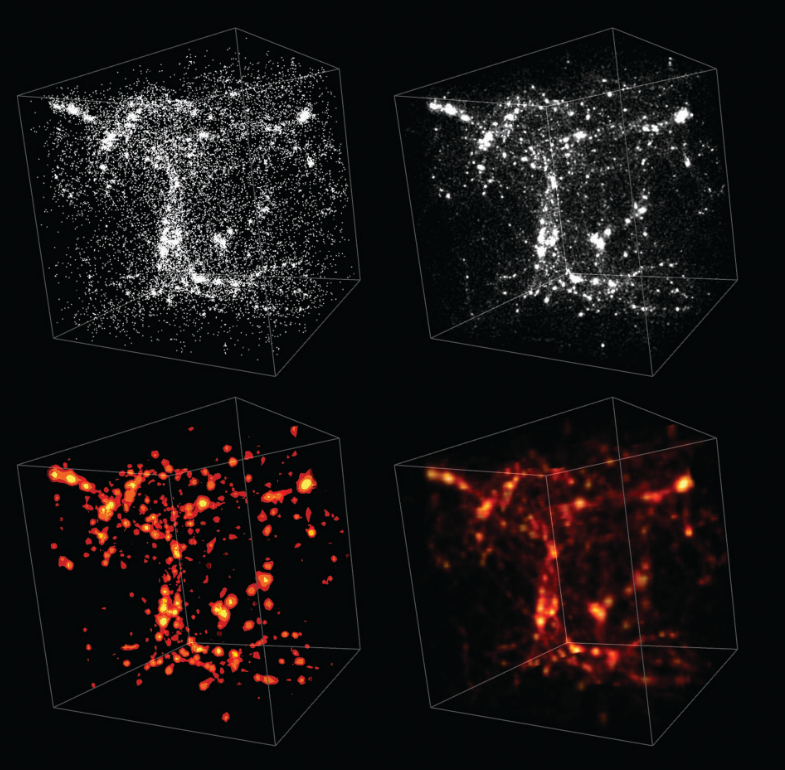
\includegraphics[width=\linewidth]{figures/visualisation.png}
    \caption{Four visualisations of an astronomy dataset using the common visualisation techniques~\cite{Hassan2011}, clearly depicting how the different visualisation techniques affect the presentation of the data. Point (top-left), splats (top-right), iso-surface (bottom-left), and volume rendering (bottom-right).}
    \label{fig:visualisation}
\end{figure}

\paragraph{Points}
% points
%   approach is limited by the available resolution (or pixeldensity) of the display
Each point in a dataset represented as a fixed-width pixel to a picture plane as if it were a three-dimensional scatter-plot.
While it is the most straightforward technique for representing data, this approach is limited by the available resolution or pixel density of a display.
This is not a suitable method for visualising astronomical data.
Simply plotting the data as a three-dimensional scatter plot makes it difficult to derive meaning from the data visualisation.
For example, the top left quadrant of Figure \ref{fig:visualisation} when compared to the bottom right quadrant is much less semantically comprehensible.

\paragraph{Splats}
This visualisation technique uses small two-dimensional textures to represent data points, and uses a method known as ``bill-boarding"~\cite{Taylor2015}, to ensure the textures always point towards the camera regardless of the scene's orientation.
When many splats are combined, this produces an effect that is much like volume rendering, but without the computational overhead of ray-tracing.

\paragraph{Iso-surface}
Polygon-based rendering, also referred to as surface rendering, is used to visualise volume data using polygons.
% three-dimensional equivalent of contouring
The majority of three-dimensional models use this method to represent their forms.
Surfaces or polygons must be extracted from volume data before it can be visualised.
Part of the visualisation process involves determining where the boundaries of the objects are and defining a skin for each region.
There are various methods for calculating these boundaries, such as: marching cubes, marching tetrahedra, multi-resolution iso-surface extraction, and surface wave propagation.
%   methods for calculating an isosurface from a data-set (check source for citations of the different methods)
Iso-surface rendering is commonly used to search for correlations between different scalar values, but is not used as a visualisation method because the visualisation is not comprehensive enough for knowledge extraction.
%   usually used to to searcg for correlation between different scalar values but are not as good at giving the overall picture of the dataset
% transparency is difficult
% boundaries could leave out interesting structures

\paragraph{Volume Rendering}
This technique renders each data point as three-dimensional pixels, also referred to as voxels. 
Voxels are arranged on the x-, y- and, z-axes to construct a three-dimensional image.
To make these structures more comprehensible, a colour transfer function is used to assign an opacity and colour to each voxel.
% volume rendering
%   provides a global view of the data-set
%   renders the external surfaces as well as the internal three-dimensional structure
%   ability to display weak or fuzzy surfaces
%   uses colour transfer function to assign an opacity and colour to the voxels
% uses ray-tracing or ray-marching shaders which can be computationally expensive
Volume rendering uses ray-tracing or ray-marching shaders to render the visualisation.
These types of shaders use significantly more computing resources compared to the traditional shading model~\cite{Wittenbrink2000}.
There are several optimisations and acceleration techniques that can tailor the shader to data being visualised.
% various algorithms for volume rendering
% back-to-front
% front-to-back
% shearing
% ray-casting
%   casts a ray from each pixel on the screen into the volume data along the viewing vector until it accumulates an opaque value
% ray-tracing
%   ray tracing is referred to as the process where reflected and transmitted rays are traced
However, it is a favoured method for representing volume data as it produces a complete view of the external surface as well as the internal three-dimensional structures within the dataset.

\subsubsection{Two-dimensional versus Three-dimensional Visualisations}
Three-dimensional visualisation techniques are better-suited for representing volume datasets, compared to two-dimensional visualisation techniques.
% why 3D is better suited for astronomy data than 2D visualisations

Some intuitive understanding of the data is missed when the data is examined using two-dimensional approaches~\cite{Kent2013}.
These approaches examine pieces of the data, such as individual slices from the dataset, or are played through sequentially like a movie.
This method of examination does not allow the user to observe the dataset as a whole.
% an intuitive understanding is missing when only examining data visualised with 2D approaches
% approaches where the iundividual channels or slices of a data cube are examined seperately 
Three-dimensional visualisations highlight hidden features within the data that would otherwise have remained hidden~\cite{Ferrand2016}.
% 3D vis techniques highight hidden features within the data that would have otherwise gone unnoticed
Comprehensive visualisations are important for communicating results quantitatively.
Therefore, visualisation which represent the data in a more comprehensive way is preferred.
% visualisation is important for communicating results quantitavely

%%%%%%%%%%%%%%%%%%%%%%%%%%%%%%%%%%%%%%%%%%%%%%%%%%%%

% challenges for petascale astronomy era
% \cite{Hassan2011}
% support of quantitative visualisation
% effective handling of large data-sets
% discovery in low signal-to-noise data
% better human-computer interaction and ubiquitous computing
% better workflow integrtion
% encouragement of adoption of 3D scientific visualisation techniques

%\cite{Hassan2011} % allow analysis to see the underlying large-scale structures hidden in the volumetric data set 
% by colour coding the points or applying a surface function to the data

% \cite{Sneiderman1996}
% mantra: overview first, zoom and filter, then details on demand
% seven data types (one-, two-, three-dimensional data, temporal and multi-dimensional data, and tree and network data)
% seven tasks (overview, Zoom, filter, details-on-demand, relate, history, and extracts).
% Exploring information collections becomes
% increasingly difficult as the volume grows.
% but the opportunity for dynamic displays takes user interface designers well beyond current wisdom. -> VR section in visual analytics
% Overall, the bandwidth of information presentation is potentially higher in the visual domain than for media reaching any of the other senses -> visual analytics section
% Users can scan, recognize, and recall images rapidly, and can detect changes in size, color, shape, movement, or texture

% \cite{Shneiderman2008}
% the purpose of visualising is insight not pictures
% the heart of information visualization is the well-designed user control panel and interaction techniques that enable users to generate task-related comprehensible coordinated windows
% The successful tools support a process of information-seeking that leads to important insights
% The successful visualization tools apply carefully designed data structures that run in the high speed store (RAM), so that even users of laptops with a few gigabytes of RAM can interactively explore million record databases.
% millions of records can translate to millions of data points within a volumetric dataset
% Billion record databases will require compression strategies or innovative hierarchical data management
% Precomputing of anticipated data needs can dramatically improve the user experience.

% \cite{Kaufman1996}
%  Volume visualization is a method of extracting information from volumetric datasets through interactive graphics and imaging, and is concerned with the representation, manipulation, and rendering of these datasets
% Volume data are 3D entities that may have information inside them, may not consist of surfaces and edges, or may be too voluminous to be represented geometrically.
% The primary sources of volume data are three: sampled data of real objects or phenomena, computed data produced by a computer simulation, and modeled data generated from a geometric model
% Examples of applications generating sampled data are medical imaging (e.g., CT, MRI), biology (e.g., confocal microscopy), geoscience (e.g., seismic measurements), industry (e.g., nondestructive inspection), and chemistry (e.g., electron density maps)
% volume cell (voxel for short), with each voxel being a rectangular cuboid havingsix faces, twelve edges, and eight corners.

% \cite{Kaufman1993}
% volume visualisation is a method for extracting meaningful information from volumetric datasets through the use of inteactive graphics and imaging. \cite{Rosenblum1994}
% provide mechanisims for peering inside volumetric datasets
% 3D voxel is the counterpart to the 2D pixel

% \cite{Rosenblum1994}
% that is, the basic ide a of using c omputer-generated pictures to gain information and understanding from data (geometry) and relationships (topology)


\subsection{Rendering}
\label{sec:rendering-strategy}
% strategies for rendering large amounts of data without storing it on the client computer
The visualisation of large amounts of data becomes problematic when processing the data consumes all of the computational resources of a non-specialised system. 
This is because the resource requirements for processing increase with the size of the data-sets~\cite{Shneiderman2008}. 
Visualisations of large data cubes can still be produced by systems with specialised hardware, but these systems are often limited by their connection to a single geographical location and restricts the number of users able to access the system at a given point in time.
% yanG2017 every line has a source in this bloody paper - refer for more sources
% visualisation is essential to make sense of the data
Visualisation of data is essential to acquire an understanding of it~\cite{Yang2017}. 
Additionally, making the visualisation interactive increases its effectiveness. 
The addition of interaction increases computational overhead as the dataset being visualised must be rendered for each frame displayed.
Changes in the visualisation's appearance resulting from interactions should be perceived as instantaneous. 
Developing a system for producing interactive visualisations of gigantic datasets in real-time is a challenge because hardware will always be pushed to its limits. 
Waiting for hardware technology to catch up with the size of the datasets is futile, as the datasets also increase in size at a steady rate over time.
The increasing size of the datasets can be attributed to many things, but specifically in astronomy it stems from data-capturing instruments becoming more sensitive and more accurate.
To solve this problem would require a system which can scale consistent performance with the ever-increasing datasets without relying on the brute-force strategy for producing visualisations~\cite{Ali2016}.
In the brute force strategy, every single data point within the dataset is visualised regardless of the size of the dataset.

While visualising the entire dataset produces a highly accurate depiction of the data, the amount of time it takes to produce the visualisation is directly linked to the computational power of the hardware.
It could potentially take a long period of time to produce the visualisation if the visualisation is produced on lower-powered hardware~\cite{Fisher2012}.
The length of time can be affected by hardware issues such as system bandwidth, which depends on factors such as the graphical computations, the speed of the display hardware, and the speed at which information can be passed between components~\cite{Becker1987}.
All of the factors present bottlenecks where system performance is potentially stunted.

The rendering speed of the visualisation is crucial to user experience~\cite{MacKenzie1993}, especially in the context of VR, where if the time between updates takes too long it could cause simulator sickness in the user, making the system unusable from the user's perspective. % look for simulator sickness source
For devices with lower-powered hardware to be able to process and visualise the data without negatively affecting system performance the dataset must be reduced in size to reduce the amount of time required to produce a visualisation.
Either through breaking the dataset up into smaller pieces~\cite{Masiane2019, Li2016} or using some sort of data reduction technique to reduce the overall resolution of the dataset through downsampling techniques such as filtering, clustering and sampling~\cite{Masiane2019, Glueck2014}. 

There are problems with both of these approaches.
Dividing the data cube into subsections has the potential to affect the integrity of the data and obscure the context of a section within the larger dataset \cite{Abidi2017}. 
Downsampled data does attempt to preserve as much detail as possible \cite{Dumitrescu2019}, although the integrity of the data cube is affected and some data can be lost.
If the time reduction provided by downsampling the data obscures potential insights, the visualisation becomes useless.
Both of these techniques reduce the accuracy of the visualisation.

The accuracy with which the visualisation is depicted in is incredibly important to the analysis of the data, as discussed further in Section \ref{sec:visual-analytics}.
It is advantageous to give the user a high-level overview of the data at the start if their workflow\cite{Li2016, Lowe2020, Zhao2017}.
This overview can be a downsampled version of the data, which would reduce the processing time because there is less data to be visualised overall\cite{Masiane2019}.
The user must be able to dig deeper into certain areas of interest in order to explore the dataset and uncover insights.
In the architecture of the astronomy visualisation system i-Davie \cite{Marchetti2020}, the user is initially presented with a downsampled version of a data cube and can then explore smaller sections at higher levels of resolution.
i-Davie was made for the exploration of data cubes on a VR device, but the majority of the computation is performed on a co-located computer, typically with mid-range computational power and a GPU.
The i-Davie system workflow is as follows, the user explores the initial data cube and finds an area of interest they would like to explore further.
The user selects that area and crops the section.
i-Davie fetches the higher-resolution version of the selected portion of the data cube.
The user sees these intermediate results at the early stage of the data processing, which allows them to do further exploration based on current knowledge.
This method of progressive visualisation facilitates the exploration of large data cubes.
It allows for speedy access to a visualisation and minimises processing time~\cite{Zhao2017} while also maintaining the accuracy and integrity of the data \cite{Masiane2019}.
% The user sees partial results at the early stage of the data processing and allows them to do further exploration based on a current view to extract knowledge from the data \cite{Zhao2017}.
This method provides required data on demand but does not overwhelm the user with too much information at once.
Even if it is a subsection of the larger data cube the context of the piece of data is understood.
The user understands how that particular section relates to the whole data cube.
This rendering strategy supports the user workflow~\cite{Hassan2011},
initially presenting the user with the full-resolution visualisation does not have a significant improvement to knowledge extraction as, the level of detail visible on the display is limited by the display's resolution. 
The visualisation wastes computational resources by attempting to render points which corresponds to an area smaller than a pixel on the chosen display hardware.
% --------------------------------------------------------------------% what is remote rendering
\subsubsection{Remote Rendering}
The remote rendering strategy is an approach to rendering which offloads computational overhead from lower-powered hardware, such as a laptop or personal computer, to higher-powered hardware, such as a dedicated server.
It makes use of the client-server model;
the server component stores the large data-sets and performs the computationally expensive processes,
whereas the client provides input as requests to the server and displays the output of these requests to the user.
This makes it possible to produce visualisations of datasets which are larger than the client's resources can accommodate~\cite{Hassan2011}.
For remote rendering to function as intended, the client must be able to access any portion of the dataset, and the server and client systems must coordinate with each other to render and display the visualisations in real time~\cite{Glueck2014}.
There are also bottlenecks present in this approach that must be considered.
% network is the biggest bottleneck - want to minimise the overall amount of data sent from server to client as well as the client to the server
The largest bottleneck is the amount of data than can be sent through a network channel in a period of time~\cite{Abidi2017}.
To mitigate the bottleneck the amount of data transferred between the server and client systems needs to be minimised.
% compression is the most common method for counteracting this bottleneck
Compression is the most common method for reducing the bottleneck.
However, compression and decompression consumes CPU on both the client and the server systems and adds time to the rendering process.
It also presents the added chance of losing data during the compression-decompression process.
The system would use lossy or lossless compression, depending on the type of data and how important the integrity of the data is to the functionality of the system.

There are two rendering strategies present in remote rendering; server-side and client side rendering, both of which are prevalent in web application development.
Systems choosing an appropriate approach for their system architecture must consider which strategy would compliment the functionality of the system ~\cite{Iskandar2020}.
% comparison between client-side and server-side rendering in web development
% software architecture
%   choose the right architecture pattern to use to maximise/optimise the utilisation in the given context the application will be used
%   different architectural patterns
%       layered, client-server, master-slave, pipe-filter, broker, peer-to-peer, event-bus, model-view-controller(layered), blackboard, interpreter
% server-side - better search engine optimisation
% client side - better user experience

\paragraph{Client-side Rendering}
% request, download bundle, extract bundle being the web application
In client-side rendering, data is downloaded from a server and then rendered in the client browser.
More specifically, in a web application a request is made to a server, a bundle of data is downloaded.
Once the bundle reaches the web application it extracts the data from the bundle and uses the data in application.
These types of applications use API calls or WebSocket connections to request a from servers.
The process of rendering of volumetric data is the same, data is stored on the server, the data is bundled and sent to the client, the data is extracted and then rendered to produce a visualisation on the client system.
% reduces latency but affects/reduces accuracy
This reduces processing time by rendering the data on the client system.
The compression and decompression of the data during the transfer process can affect its accuracy.
The integrity of the data could also be affected by the downsampling process it went through on the server..
The amount of data that can be rendered is limited to the computational power of the client system while the client system performs other tasks besides those related to the rendering of the data visualisation~\cite{Becker1987}.
In a comparison between client-side and server-side rendering, client-side produces a better user experience~\cite{Iskandar2020}, as the interactions performed on the client are perceived as instantaneous.

\begin{figure*}
    \centering
    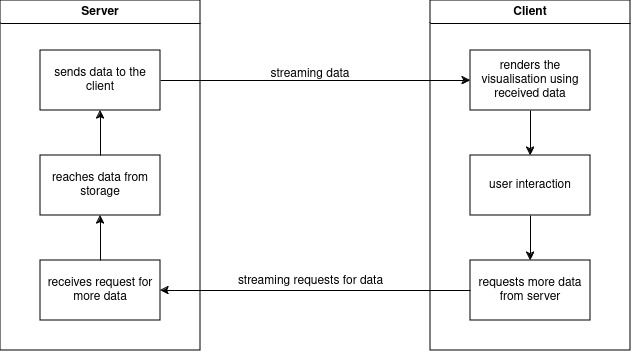
\includegraphics[width=0.6\linewidth]{figures/client-side-rendering.jpg}
    \caption{An example of the process of client-side rendering where data is sent from the server to the client to be rendered. The user interacts with the data on the client and only requests more data from the server when it is required.}
    \label{fig:client-rendering}
\end{figure*}

\paragraph{Server-side Rendering}
% Server side rendering is were static or semi-static web-pages are hosted on a server, and when the user opens a websites these pages are sent from the server.
Server-side rendering involves storing the data on the server and also rendering the data into a visualisation on the server.
Frames of this visualisation are sent to be displayed on the client web application.
% server handles requests from the client, performas actions, and returns a response
The client system has no part in the rendering process, it just displays the frames it receives from the server. 
The user can manipulate the visualisation by forwarding input capture by the client application to the server, following the classic request-response model for web applications.
% In remote visualization (or remote computation) heavy graphics tasks are delegated to a high-end graphics server that actually performs the 3-D rendering and generates a 2-D frame that can be visualized on a remote device (possibly characterized by limited hardware resources). 
The server renders the three-dimensional visualisation of the data but streams two-dimensional images to the client.
% Server-side rendering is implemented when there are computationally expensive graphics tasks that need to be performed.
% These tasks are delegated to the server which has enough computational resources to perform them, whereas the client system does not have the hardware resources to produce the visualisation~\cite{Becker1987}.
% increases accuracy but increases latency 
This strategy increases the accuracy as the integrity of the data is unaffected as it is not processed or transferred, however, it does increase processing time.
The main point where this processing time becomes apparent is when the user performs interactions with a visualisation on the client system.
The user must wait for the interaction to be forwarded to the server, then the visualisation must be re-rendered, and finally the updated frames are streamed to the client.
The time in which these tasks are done increases if the frames are also compressed for transfer over a network, and subsequently decompressed on the client.
The speed of the network the frames are streamed on also affects the processing time of the feedback to the user on the client system.
The slower the network, the more time the user has to spend waiting for feedback.
The server could also have a delayed response because it is performing other tasks, and handling many clients' requests~\cite{Becker1987}.

\begin{figure*}
    \centering
    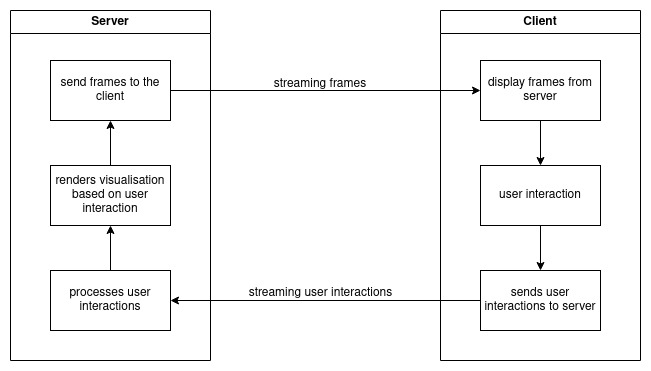
\includegraphics[width=0.6\linewidth]{figures/server-side-rendering.jpg}
    \caption{An example of the server-side rendering process, where the rendering of the data is done on the server and the frames are streamed to the client. The user interacts with the visualisation on the client but the interactions are sent to the server. The rendering is updated based on the user interactions and the frames are once again streamed to the client.}
    \label{fig:server-rendering}
\end{figure*}
\subsection{Current Visualisation Systems}
\label{sec:current-systems}
Extremely large datasets are commonplace within radio astronomy research. 
As this research progresses, the datasets are predicted to balloon in size even more at ever faster rates.
Advances in astronomical technology, such as larger detectors, increases in bandwidth, and astrophysical simulations, drive the need for visualisation solutions.
Specialised systems have been developed to cater to this aspect of astronomy data, as well as to astronomy researchers. 
While not all of these systems attempt to apply a generalist approach to volumetric data visualisation, important points can be taken from the systems reviewed.
The system architectures and strategies employed to handle the enormous amount of data produced by modern radio astronomy data-capturing instruments emphasise points that can be applied to various systems, as there are some shared goals.
Sources~\cite{Ferrand2016, Hassan2011, Naiman2016, Kent2013, Shneiderman2008} highlight a need for a generic standalone, cross-platform application capable of processing and visualising large amounts of volumetric data. 
These visualisations, used in addition to traditional statistical visualisations, have complementary effects on knowledge extraction by communicating information clearly and effectively~\cite{Caldarola2017, Goodman2012, Naiman2016, Rosenblum1994} especially as the variety of data grows and becomes more complex.
% want for a cross platform appication capable of processing and visualising various types of astronomy data formats, especially as those format grow evermore complex

\subsubsection{Big Data Visualisation Systems}
While not specifically geared towards astronomy data visualisation, these systems face similar issues handling large amounts of scientific data, and reviewing some of these systems could add valuable insight which can be applied to the development of radio astronomy visualisation systems.

% The big data era has made many very large datasets available, they are dynamic and characterised by high variety and volitility where new data is constantly being added
\textit{Big data} as a term can be defined as ``datasets whose size is beyond the ability of software tools to capture, store, manage, and process''~\cite{manyika2011, Sneiderman1996} or ``data which exceeds the capabilities of commonly used hardware environments and software tools to capture, manage, and process it within a reasonable amount of time''~\cite{merv2011}.
These datasets have characteristics relating to the three V's of \textit{big data}: volume, velocity, and variety.
As volume increases, problems involving processing, storing, and extracting knowledge arise.
When variety increases it complicates the storage and analysis of the data because of the different structures of data being stored.
Velocity relates to the speed at which data is generated, this has the potential to compound the issues of storing and processing a high volume of data~\cite{Caldarola2017}.
This is because processing data takes time and if data is not process fast enough it creates a backlog when new data is inbound.

There are various software packages and platforms to assist the user in making sense out of massive amount of information, each tailored to a specific use case.
For big data visualisation and analytics, great consideration must be put into the method of visualisation because the structure of the data affects the resulting visualisation.
Generally the tools value flexibility and user convenience.
By making these tools available on multiple platforms for ease of access and by having them be programming language agnostic, allowing the user to cutomise their workspace.
% There is a wide range of data plotting software that can be used to tailor a solution according to the data that needs to be analysed.
% RNeo4J, Statnet, Tableau, infogram, Tulip

A general solution to visualisation and analytics is complicated because it is impossible to account for all methods of visualisation and for the variety of data.
But most are aimed towards business analytics.
Some examples of data visualisation software for specific data types are:
\begin{itemize}
  \item Timeline - specialised to create interactive timelines from a spreadsheet
  \item Commetrix and Cuttlefish - used for dynamic network visualisation and analysis
  \item Cytoscape - used for visualising molecular interaction networks and biological pathways, originally designed for biological research but is now also used for complex network visualisation and network analysis
\end{itemize}

Current systems used for exploration and visualisation cannot handle the size of many contemporary datasets and restrict themselves to analysing only comparatively small data-sets.
This is mainly due to them using a brute force method of visualising the entire dataset regardless of how it will appear on a display~\cite{Bikakis2018}.
% offline - use a single local machine to generate the visualisations

The free-to-use game engine Unity~\cite{Marchetti2020, Ferrand2016, Ferrand2018} and the open source three-dimensional modelling and animation software Blender~\cite{Taylor2015, Taylor2016, Kent2013, Naiman2016} have been used for fast prototyping of various astronomy visualisation systems.
Blender is favoured for three-dimensional rendering capabilities and it three-dimensional space manipulation tools,
particularly useful for generating animations and graphics with astronomy data.

\paragraph{ParaView}
ParaView~\cite{Ahrens2005}, is an example of a tool created for scientists to visualise and analyse extremely large data-sets,
while emphasising the workflows of the domain experts.
It highlights speed and performance as key aspects of the software's functionality.
Its rendering strategy involves executing programs in parallel on either shared or distributed memory resources.
% supports hardware accelerated parallel rendering
% acheives interactive rendering performance via level-of-detail techniques
It can achieve high frame rates suitable for interaction by utilising level-of-detail techniques.
These level-of-detail techniques, also known as progressive visualisation, involve storing the dataset at many different resolution levels, which are also know as mipmaps.
They reduce the amount of data that has to be rendered, which also impacts the quality of the visualisation.
The dataset being visualisation must find a balance between the resolution of the data and the performance of the system
%  advantage of progressivly refining a coarse model of the data
% But leveraging the advantages of refining a coarse model of data and refining parts as the user works through the data.
\begin{figure*}
    \centering
    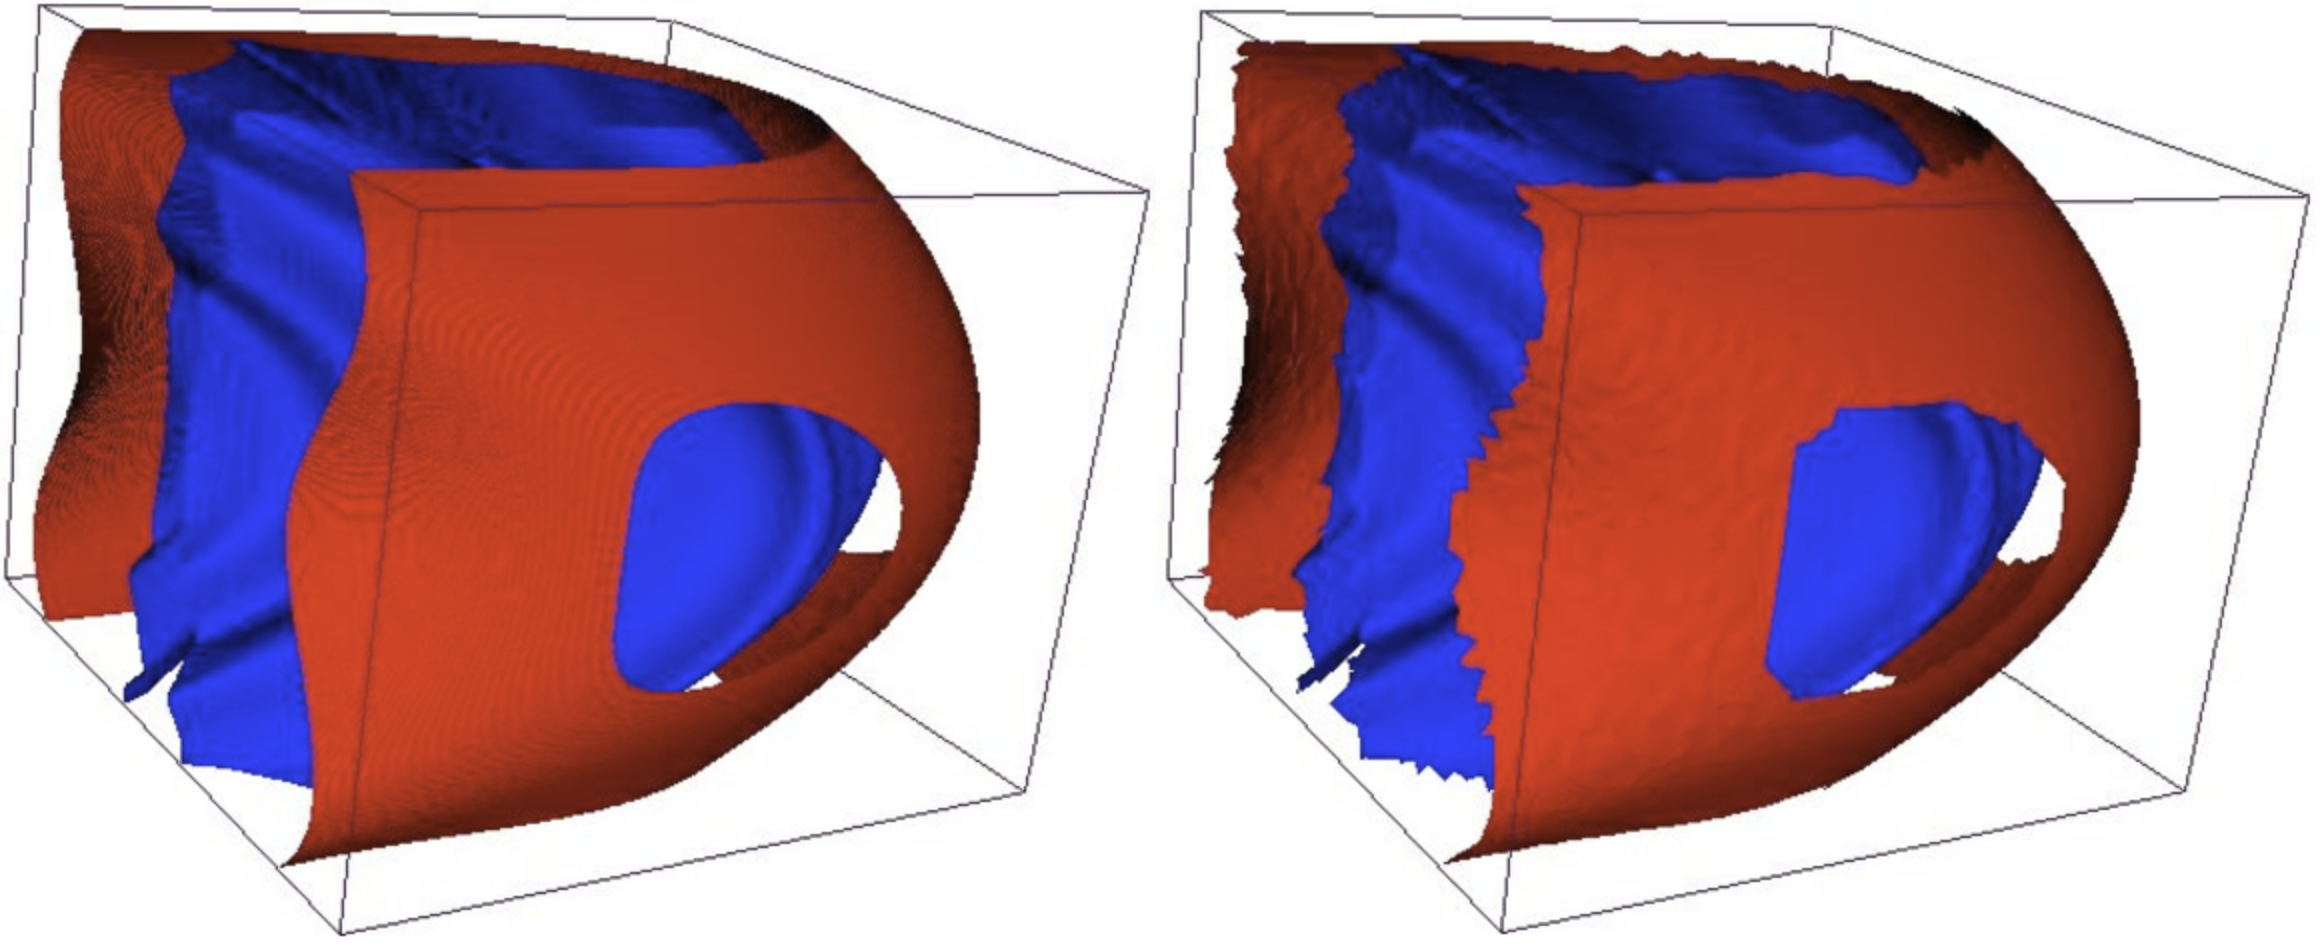
\includegraphics[width=0.6\linewidth]{figures/paraview.png}
    \caption{An example of a level-of-detail technique specified by ParaView. The model on the left is rendered at a higher resolution than the one on the right. While the quality of rendering is impacted, but improving rendering performance by having a lower resolution model to visualise.}
    \label{fig:paraview}
\end{figure*}
% multi-resolution representations or mipmaps as well as parallelism can be used to improve both visualisation and rendering performance
% describing and exploratory mode (a graphical user interface toll is used to explore the dataset) and batch mode (scripting and programming languages are used to write and execute a program

% portability - for to function on the diverse computational resources available and differnt displays (VR)
% accessability - ability to gain access to, setup, and run the tool
% extensibility - ability to easily add new functions to the tool
% describes a large dataset as data that exceeds the resource limit of a single machine
% uses a layered architecture
ParaView uses a layered architecture~\cite{Ahrens2005}.
The VTK foundation layer handles the data representation and algorithms~\cite{Ahrens2005}.
The second layer handles the parallel extensions to the visualisation toolkits, while supporting streaming of many data types and parallel execution.
The third and final layer is ParaView itself, which provides a graphical user interface and the visualisations.

\subsubsection{Astronomy Data Visualisation Systems}
Among the systems used to process and visualise \textit{big data} datasets there are some systems exclusively made for astronomy data.
% \cite{Lan2021}
% a comprensive catalogue of the current state of visualisation technologies present in astrophsyics

\paragraph{CARTA}
The acronym CARTA stands for Cube Analysis and Rendering Tool for Astronomy~\cite{Comrie2021}.
% aim is to provide a usable and scalable system utilising modern web technologies and parallel computing
Its objective is to provide a usable and scalable system using modern web technologies,
and its main hallmark is being able to load and render a dataset of several Terabytes in a matter of second.
It achieves this by storing the dataset at various levels of resolution and sending only the required requested data to produce a comprehensible rendering, instead of attempting to render the whole dataset at once.
% hosts large datasets remotely, uses the remote approach
It makes use of the client-side remote rendering approach for handling large datasets, by hosting them on a remote server.
% access the remote data from a local web-based client
A local web-based client accesses the data through a network connection, the data is transferred to the client and rendered within the web browser.
% focuses on being able to load a dataset of several TeraBytes worth of data in a matter of seconds
% designed for the ALMA, VLA, SKA pathfinders
It is designed for the ALMA, VLA, and SKA pathfinders
% works with data types such as FITS, CASA, MIRIDA, and HDF5
and works with data types commonly used in astronomy research such as FITS, CASA, MIRIAD, and HDF5.

\paragraph{i-DAVie}
This software for data cube exploration within a virtual environment, 
providing tools to navigate and interact with the visualisations.
Functionality to view metrics and interactively mask regions of data in the VR environment to catalogue sources is particularly useful.
% They enable a unique and immersive perspective on the data and allow intuitive interactions with the data
The VR environment integration enables a unique and immersive perspective of the data, affording intuitive interactions.
% created using the Unity game engine
It was created using the Unity game engine and uses the client-server architecture within its design~\cite{Marchetti2020}.
% system design uses the client-server model with server side rendering, where the visualisation is generated on the server and the frames are streamed to the front-end
It stores the datasets on the server but also renders the visualisation using the server.
% takes computational load off of the client but adds latency to the inteactions
% This approach takes computational load off the client but adds latency to the visualisation feedback as the user interactions must first be sent to the server, then visualisation is then updated based on the received interaction, and finally the frames are sent back to the client.
% The latency is proportional to the distance the client is from the server, and therefore latency increases as the distance between the client and server increases.
%   interactions performed on the client is sent to the server
%   visualisation is udated based on the input
%   frames are sent back to the client
A prototype system similar to i-Davie created for public outreach~\cite{Ferrand2018}, is a tethered standalone system which means that the server and the client are connected to each other with a physical connector such as a cable.
It also uses Unity with custom scripts to visualise FITS files and displays the visualisation in a VR environment using the HTC Vive. 
It can produce iso-surface or volumetric visualisations of a dataset.

\paragraph{Frelled}
A general-purpose astronomy viewer~\cite{Taylor2015} which uses a set of Python scripts to create three-dimensional visualisations of FITS files inside Blender, and is used for visual source extraction, cataloguing, and analysis.
It can visualise large datasets of roughly 600,000 points at more than 10 frames per second, while providing tools to mask data interactively, functionality similar to i-DAVie.
The FITS file can be explored in a three-dimensional space, instead of two-dimensional slices.
It provides a significant speedup in source cataloguing compared to other viewers, facilitating the recording of hundreds of sources a day.
Visual source extraction by an astronomer is still currently more effective than automated processes.
% motivations
%   desire to view 3D datasets in a 3D space
%   the need to rapidly mask regions of the data

\paragraph{AstroBlend}
A Python package for Blender~\cite{Naiman2016}, combining the three-dimensional capabilities of Blender with astronomy analysis tools.
Allows astronomers to analyse data alongside visualisations, while simplifying the importing process.
% simplifies the importing process of importing astrophysical datasets, generating visualisations, and anyalysis plots

\paragraph{SlicerAstro} % other good sources
A multi-platform open-source package for visualising and processing medical images,
which is an extension of the open-source software 3D slicer~\cite{Fedorov2012}.
It aim is to provide an interactive three-dimensional visual analytics tool using two-dimensional displays and interaction devices.
It is implemented using C++.
Its features include interactive filtering, three-dimensional masking and modelling, and support for FITS files.

\paragraph{E0102-VR}
\cite{Baracaglia2019}
An experimental standalone application using a VR display and interaction devices.
Its aim is to demonstrate the benefits of using human depth perception for fast and accurate characterisation of three-dimensional structures.
It explores the scientific potential of VR for displaying multi-dimensional datasets in astronomy and astrophysics.
The system pre-processes datasets into an iso-surface representation as it does not currently support volume rendering.
These pre-processed datasets can be swapped out with no effect on the functionality, but the system is currently coupled to a single dataset (SNR E0102) for experimental purposes.
The size of the dataset is limited because all the computation is done on a single computer.
% the pre-compiled/pre-processed dataset can be swapped out with no major loss of functionality
%   currently coupled to a single dataset (SNR E0102) for experimentation purposes
% uses isosurfaces to represent the visualisation
% limits the size of the datasets that can be used as all computation is done on a single computer
\subsection{Findings}
\label{sec:findings}
% VR findings
Virtual reality technology has made significant strides since its conceptualisation, evolving into immersive experiences that blur the lines between real and virtual environments. 
Central to the effectiveness of VR experiences are the concepts of presence, interactivity, and immersion. 
Presence is the sensation of physically existing within the virtual world, influenced both by subjective perceptions and objective indicators. 
Interactivity allows users to engage dynamically with the virtual environment, enhancing their sense of immersion and agency. 
Immersion, with its cognitive, emotional, kinesthetic, and spatial dimensions, contributes to a rich user experience across various platforms. 
Challenges such as simulator sickness highlight the importance of high-performance hardware in maintaining immersion and preventing adverse effects. 

% interaction is also very important in visual analytics
% interaction creates a much deeper experience for the user whether it is for entertainment or knowledge extraction

% Thus, interactivity serves as a crucial determinant of the overall quality and effectiveness of the user experience, shaping the user's sense of presence, immersion, and agency within the digital realm.
% Simulator sickness can affect some individuals but can be diminished 

% visual analytics key findings
% progressive rendering benefits both rendering effeciency and visual analytics

% The user explores the data from a broad overview and refines there search through continually adjusting the subset of data as they explore.
% From a system efficiency perspective the broad overview is a down-sampled data cube and as the user explores higher resolution portion of the data-set is brought to be visualised.
% Decreasing the time which the user is waiting for the visualisation as well as decreases the computational load on the system by limiting the amount of data visualised at any point in time.

The integration of visual analytics into data exploration and analysis practices offers a dynamic approach to uncovering insights and patterns within datasets. 
Through visual representations, analysts are empowered to interact with data, leveraging their inherent pattern recognition abilities to extract knowledge effectively. 
% For a data-set to be explored effectively there must be some way of interacting with it to facilitate exploration.
% This is to aid in extracting knowledge from the visualised data-set, and is imperative to the users ability to extract data from a visualisation
% Whether exploring to construct hypotheses, analysis to validate conjectures, or presentation-focused visualisation for effective communication, 
The goal of visual analytics is to enhance analytical reasoning and research through interactive visualisations. 
The efficacy of visual analytics hinges on user interaction, where progressive visualisation plays a pivotal role. 
It benefits both the flow of exploration for the user as well as the overall functionality of the system.
By allowing users to steer the representation's progress through data exploration, it facilitates a seamless transition from low-fidelity overviews to detailed insights. 
This iterative process, supported by techniques such as zooming, filtering, and immersive experiences like VR, enables analysts to navigate complex datasets efficiently. 
VR offers a compelling avenue for immersive analytics, providing an intuitive environment for multi-dimensional visualisations. 
By bridging the gap between quantitative data and human perception, VR not only enhances interaction but also enriches the understanding of complex phenomena, fostering a more holistic and user-centric approach to data analysis.

% data visualisation key findings
% explores how volumetric data can be rendered on a display
% Volumetric data can be represented as a visualisation using many different techniques, such as points, splats, iso-surfaces, and volumetric rendering.
% Each technique varies in how much computational resources is required to generate a visualisation.
% compares techniques such as points, splats, iso-surfaces, and volumetric rendering to determine the positives and negatives of each method
The data visualisation section \ref{sec:data-visualisation} also discusses the benefits of of using a three-dimensional visualisation rather than two-dimensional views. 
The visualisation of volumetric data cubes, particularly in fields like astronomy, presents a challenge because the complexity and scale of the datasets involved. 
These data cubes are essential for understanding phenomena in various scientific disciplines, including astronomy, medicine, oceanography, molecular-modeling, and engineering. 
Visual representation techniques unlock insights from these datasets.

One of the key objectives of data visualisation is to enable users to explore and understand complex data more deeply while having the means to communicate their findings to others. 
However, the unique characteristics of radio astronomy data, such as its massive size and dynamic range, present specific challenges for visualisation.

Various visualisation techniques exist, each with its own advantages and limitations. 
These include points, splats, iso-surfaces, and volume rendering. 
Among these, volume rendering emerges as the most comprehensive method for representing volume data, providing a detailed view and of external surfaces and internal structures within the dataset. 
It is resource-intensive, volume rendering offers a robust approach for extracting knowledge from volumetric datasets.

Furthermore, the choice between two-dimensional and three-dimensional visualisations is crucial. 
While two-dimensional approaches may be enough for certain analyses, three-dimensional visualisations are generally more effective for representing volumetric datasets comprehensively. 
They reveal hidden features and allow for a more intuitive understanding of the data, enhancing communication of quantitative results.

In summary, effective visualisation techniques are unlocking insights from volumetric datasets in fields such as astronomy. By leveraging advanced visualisation methods like volume rendering and prioritising three-dimensional representations, researchers can better understand complex data and communicate their findings more effectively.

% rendering strategy key findings
% In the rendering strategy section it was found that it is not enough to simply scale the computational power of a system as the size of data cubes increase, there is a need for a more intelligent strategy to handle the increasing size of the data cubes.
% It is very inefficient to simply brute-force the generation of visualisations by throwing more computational resources at the issue.
% The size of the data cubes are increasing in size at a faster rate than the development of the computational power of system, especially devices made for commercial consumption by the mass market. % see if i can find a source for the increase of data in astronomy and computer power
The rendering strategies section addresses the challenges of visualising large datasets and the strategies that balance computational efficiency with maintaining data integrity and user experience. 
Traditional approaches, such as brute force visualisation, strain computational resources and impede real-time interaction. 
To overcome these limitations, progressive visualisation techniques, used by i-Davie, offer a solution. 
By presenting users with initial down-sampled overviews and enabling them to explore areas of interest in greater detail, these methods optimise processing time without sacrificing accuracy or overwhelming users with excessive information. 
Moreover, remote rendering strategies, whether server-side or client-side, offer avenues for offloading computational overhead and accommodating datasets larger than the client's resources can handle. 
However, network bottlenecks and trade-offs between data compression and integrity must be managed carefully to ensure efficient data transfer and timely user feedback. 
As datasets continue to grow in size, the development of scalable visualisation systems that prioritise both performance and usability remains imperative.

% explore current system which work on the problem of visualising very large volumetric data-sets
% current systems key finding
% Some of the current systems that were reviewed produced some key points.
% Such as the benefits of pre-processing large datasets where the system retrieve higher detail versions of a section of data to provides a speedup with data visualisation.
% Three-dimensional representations produce a better experience for viewing multi-dimensional datasets and VR displays provide a more intuitive experience when working with multi-dimensional datasets than two-dimensional displays.
% VR technology also leverages user depth perception and spatial awareness.

% In some current astronomy visualisation systems they attempt to use datasets in the FITS file format to create 3D visualisations. 
% Implementations produce effective three-dimensional visualisations, however, the Fits file format is not suited for efficient visualisation as the data is stored in sequential slices, like pages in a book. 
% This makes traversing and extracting data to create the three-dimensional visualisation tedious. 
% Files can also be too large to be visualised as a whole and whole have to be broken up into more manageable pieces for visualisation.
% Breaking datasets into pieces runs the risk of obscuring the context of the individual piece and could obscure the insight the dataset would communicate as a whole.

% While building the experimental system E0102-VR~\cite{Baracaglia2019} some insights were found involving the use of VR for viewing and interacting with multi-dimensional datasets.
% The depth perception provided by VR aids in understanding complex three-dimensional structures and provides means to quickly measure distances and angles in three dimensions.

The review of existing systems has highlighted several key points. 
For instance, the advantages of pre-processing large datasets, where systems retrieve higher-detail sections of data to expedite data visualisation. 
Three-dimensional representations enhance the viewing experience for multi-dimensional datasets, and VR displays offer a more intuitive interface compared to two-dimensional displays. 
VR technology capitalises on user depth perception and spatial awareness, further improving the visualisation process.

Efforts have been made to utilise datasets in the FITS file format to generate 3D visualisations, in system such as \textit{Frelled} and \textit{SlicerAstro}
While these implementations yield effective three-dimensional visualisations, the FITS file format is not inherently conducive to efficient visualisation because of its storage of data in sequential slices, like pages in a book. 
This sequential storage method makes traversing and extracting data for three-dimensional visualisation a cumbersome task. 
Additionally, files may be too large to visualise in their entirety, necessitating the division of datasets into more manageable pieces. 
However, breaking datasets into fragments risks obscuring the context of individual pieces and potentially diluting the insights the dataset would otherwise convey as a whole.

During the development of the experimental system E0102-VR, valuable insights were gained regarding the utilisation of VR for viewing and interacting with multi-dimensional datasets. 
The depth perception afforded by VR aids in comprehending complex three-dimensional structures and facilitates rapid measurement of distances and angles in three dimensions.
